\documentclass[tikz]{standalone}
\include{preample}
\def\flowwidth{2cm}
\tikzstyle{start} = [rectangle,
rounded corners,
minimum width=\flowwidth,
minimum height=.75cm,
text centered,
text width=\flowwidth,
draw=black,
fill=gray!30]

\begin{document}
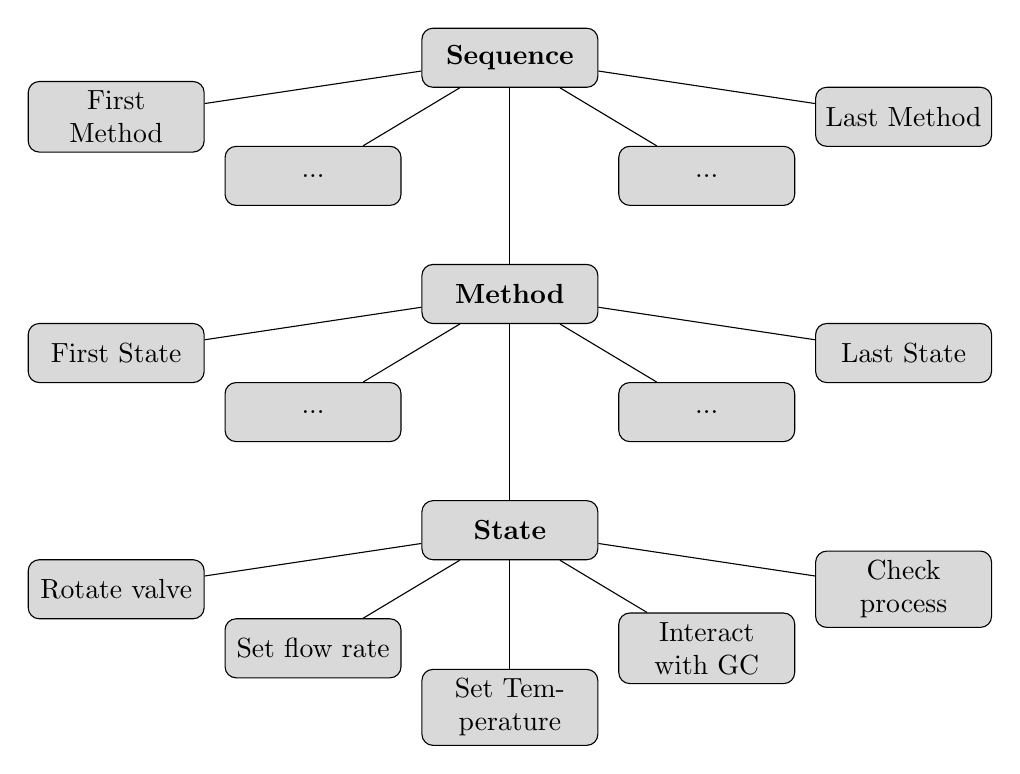
\begin{tikzpicture}[node distance=1.5cm]
    \node (seq) [start] {\textbf{Sequence}};
    %%%%%%%%%%%%%%%%%%%%%%%%%%%%%%%%%%%%%%%%
    % Methods
    %%%%%%%%%%%%%%%%%%%%%%%%%%%%%%%%%%%%%%%%
    \node (method) [start, below of=seq, yshift=-1.5cm] {\textbf{Method}};
    \node (method1) [start, below of=seq, yshift=.75cm, xshift=-5cm] {First Method};
    \node (method2) [start, below of=seq, xshift=-2.5cm] {...};
    \node (method3) [start, below of=seq, xshift=2.5cm] {...};
    \node (method4) [start, below of=seq, yshift=.75cm, xshift=5cm] {Last Method};
    %%%%%%%%%%%%%%%%%%%%%%%%%%%%%%%%%%%%%%%%
    % States
    %%%%%%%%%%%%%%%%%%%%%%%%%%%%%%%%%%%%%%%%
    \node (state) [start, below of=method , yshift=-1.5cm] {\textbf{State}};
    \node (state1) [start, below of=method,  yshift=.75cm, xshift=-5cm] {First State};
    \node (state2) [start, below of=method, xshift=-2.5cm] {...};
    \node (state3) [start, below of=method, xshift=2.5cm] {...};
    \node (state4) [start, below of=method,  yshift=.75cm, xshift=5cm] {Last State};
    %%%%%%%%%%%%%%%%%%%%%%%%%%%%%%%%%%%%%%%%
    % Controls
    %%%%%%%%%%%%%%%%%%%%%%%%%%%%%%%%%%%%%%%%
    \node (valve) [start, below of=state , xshift=-5cm, yshift=.75cm] {Rotate valve};
    \node (flow) [start, below of=state, xshift=-2.5cm] {Set flow rate};
    \node (temp) [start, below of=state, yshift=-.75cm] {Set Temperature};
    \node (GC) [start, below of=state , xshift=2.5cm] {Interact with GC};
    \node (wait) [start, below of=state , xshift=5cm, yshift=.75cm] {Check process};
    \draw (seq) -- (method1);
    \draw (seq) -- (method2);
    \draw (seq) -- (method3);
    \draw (seq) -- (method4);
    \draw (seq) -- (method);
    \draw (method) -- (state1);
    \draw (method) -- (state2);
    \draw (method) -- (state3);
    \draw (method) -- (state4);
    \draw (method) -- (state);
    \draw (state) -- (valve);
    \draw (state) -- (flow);
    \draw (state) -- (temp);
    \draw (state) -- (GC);
    \draw (state) -- (wait);
\end{tikzpicture}
\end{document}